\documentclass[runningheads]{llncs}
\usepackage[T1]{fontenc}
\usepackage{amsmath, amssymb, amsfonts}
\usepackage{bm}
\usepackage{booktabs}
\usepackage{multirow}
\usepackage{array}
\usepackage{float}
\usepackage{makecell} 

\usepackage{graphicx}
\usepackage[ruled,linesnumbered]{algorithm2e}
\usepackage[colorlinks=true, linkcolor=blue, citecolor=blue, urlcolor=blue]{hyperref}
\usepackage{listings}
\usepackage{xcolor}
\title{TEMPO: Hierarchical Phase Control Reduces Token Cost in Long-Horizon LLM Tool Use}
\titlerunning{TEMPO: Hierarchical Phase Control Reduces Token Cost}
\author{Anonymous Author(s)}

\authorrunning{Anonymous Author(s)}
\institute{Paper under Double-Blind Review}

\begin{document}
\maketitle
\begin{abstract}
ReAct-based LLM agents incur unnecessary LLM calls at every decision step, even for highly predictable tool interactions. Existing tool-inertia mechanisms address this by bypassing the LLM when a static confidence threshold is exceeded, but a single fixed threshold cannot serve the qualitatively distinct phases of long-horizon tasks: it suppresses useful inertia during routine execution and blindly reuses outdated actions at sub-task boundaries. We propose \textbf{TEMPO} (Task-Efficient Macro-action Planning via phase Orchestration), a hierarchical reinforcement learning framework built on two coupled components. First, a deterministic \textsc{PhaseDetector} — a three-state finite state machine (FSM) — segments each trajectory into \emph{Exploration}, \emph{Execution}, and \emph{Transition} phases by monitoring per-step progress signals. Second, a Semi-MDP macro-controller implemented as a DQN selects a phase-level inertia strategy at every FSM-triggered phase boundary, committing to it for the entire phase duration. This two-level design reduces RL decision frequency by aligning triggers with semantic transitions, provides denser credit assignment through phase-level rewards, and enables phase-conditioned context trimming. Experiments on ScienceWorld and AlfWorld show that TEMPO improves success rate by up to 15.6 percentage points over AutoTool while reducing token consumption by up to 42.9\% on dense-reward environments; in sparse-reward settings, TEMPO prioritises reasoning integrity over token savings.


\keywords{LLM Agents \and Hierarchical Reinforcement Learning \and Semi-MDP \and PhaseDetector}
\end{abstract}

\section{Introduction}
Large Language Models (LLMs) such as GPT-4 \cite{gpt4} and Llama 3 \cite{llama3} have established a new foundational paradigm for constructing autonomous agents capable of following complex instructions and utilizing external tools. Frameworks like ReAct \cite{react} and analytical platforms such as AgentBoard \cite{agentboard} illustrate the efficacy of the interleaved \emph{thought--action--observation} cycle for multi-turn tasks. However, a fundamental efficiency-capability trade-off persists: the autoregressive nature of LLM generation necessitates an expensive inference call at every decision step. As task horizons grow, compounding token consumption and substantial response latency severely restrict the large-scale deployment of agents in real-world domains \cite{deepseekr1,bot}.

Existing optimization strategies have predominantly focused on model distillation \cite{agentflan} or dual-system routing architectures \cite{swiftsage}. In a complementary direction, AutoTool \cite{autotool} introduced the concept of "tool-usage inertia," which bypasses the LLM when a Contextual Inertia Prediction Score (CIPS) exceeds a fixed confidence threshold $\theta$. Directly replaying frequent actions can significantly reduce inference costs; however, static thresholds fail to adapt to the qualitatively distinct behavioral regimes encountered in long-horizon task lifecycles. During early exploration, a rigid threshold often triggers inertia before a coherent plan has formed; conversely, at sub-task boundaries, blind reuse risks replaying outdated actions. In our experiments, Qwen2.5-72B’s success rate on AlfWorld dropped by 21.2 percentage points (from 86.9\% to 65.7\%) under AutoTool, highlighting a critical "phase-blind" defect that causes performance collapse in reasoning-intensive stages.

Optimal compute allocation requires both temporal consistency and macro-cognitive awareness \cite{agentlite}. Decisions made at the instantaneous step level are often noisy and struggle with sparse rewards, particularly in environments like AlfWorld where feedback remains binary until task completion. The Options Framework and Semi-Markov Decision Process (Semi-MDP) theory \cite{sutton1999between} provide the theoretical foundation for temporal abstraction, allowing agents to commit to macro-actions (options) that persist over multiple time steps. This motivates a hierarchical design where the agent distinguishes between semantic phases—Exploration, Execution, and Transition—managing its cognitive budget at the phase level rather than the step level.

We propose \textbf{TEMPO}, a hierarchical framework that models tool usage inertia control as a Semi-MDP. TEMPO integrates two core components: a deterministic \textsc{PhaseDetector} implemented as a three-state finite state machine (FSM) that segments trajectories based on per-step progress signals, and a macro-controller DQN that selects phase-level inertia strategies at semantic boundaries. By making strategic commitments at phase boundaries, TEMPO minimizes decision frequency by performing inference only at phase boundaries, supporting phase-conditioned context management to further prune redundant history that makes little or no difference to inertia calls.

The main contributions are:
\begin{itemize}
    \item \textbf{Semi-MDP Temporal Abstraction.} We model tool inertia control as a hierarchical scheduling problem, replacing noisy step-level decisions with phase-level macro-actions. By binding decisions to semantic phases, we enable "temporal commitment" that resolves policy non-stationarity in long-horizon trajectories.
    \item \textbf{Dense Credit Assignment via Phase Rewards.} We design a phase-level reward mechanism that aggregates progress gains, token costs, and inertia precision across phases. This overcomes the sparse reward bottleneck common in agents, providing a significantly denser learning signal for the controller.
    \item \textbf{Phase-Aware Macro-Perception.} We introduce 7-dimensional state summaries that broaden the macro-controller's temporal receptive field through phase-level aggregation. This allows the system to capture macro-behavioral structures and filter the instantaneous environmental noise that plagues flat RL models.
    \item \textbf{Pareto Efficiency Improvement.} Extensive evaluations across ScienceWorld and AlfWorld demonstrate that TEMPO breaks the performance-cost zero-sum game on dense-reward environments, improving success rates by up to 15.6 percentage points while reducing token consumption by up to 42.9\%.
\end{itemize}

\section{Background and Related Work}

\subsection{Architectural Evolution and Efficiency of LLM Agents}
The paradigm of autonomous agents has shifted from basic few-shot prompting to complex reasoning systems. Early frameworks like ReAct established the core loop of interleaved thinking and acting, while reasoning-intensive models such as DeepSeek-R1 and Llama 3 have extended logical depth at the cost of prohibitive inference overhead. Recent work addresses this via model distillation (Agent-FLAN \cite{agentflan}) and hierarchical sub-task decomposition (Agent-lite \cite{agentlite}), but neither targets the \emph{dynamic regulation} of computational investment within a single long-horizon trajectory.

\subsection{Optimization Strategies for Tool Learning and Tool Use}
While ToolLLM \cite{toolllm} and Toolformer \cite{toolformer} focus on tool selection accuracy, recent work prioritises reducing inference redundancy. AutoTool introduced "tool usage inertia," using static graph-based transition scores to bypass LLMs during repetitive sequences. Buffer-of-Thoughts \cite{bot} and Chain-of-Abstraction \cite{coa} similarly cache routine reasoning steps. All of these rely on fixed, context-free heuristics; TEMPO instead adapts the bypass threshold dynamically across semantically distinct task phases.

\subsection{Temporal Abstraction and Hierarchical Decision Making}
The Options Framework and Semi-MDP theory \cite{sutton1999between} provide the theoretical foundation for temporal abstraction, allowing agents to commit to macro-actions over variable time spans. Contemporary step-level routing methods such as RouteLLM \cite{routellm} and DOTS \cite{dots} suffer from high variance and sparse reward signals precisely because they decide at every step. TEMPO instantiates a Semi-MDP where a deterministic FSM identifies semantic phase boundaries, enabling macro-decisions that yield denser credit assignment and reduced policy variance.

\section{Method}
\label{sec:method}

\begin{figure}[htb]
    \centering
    \small
    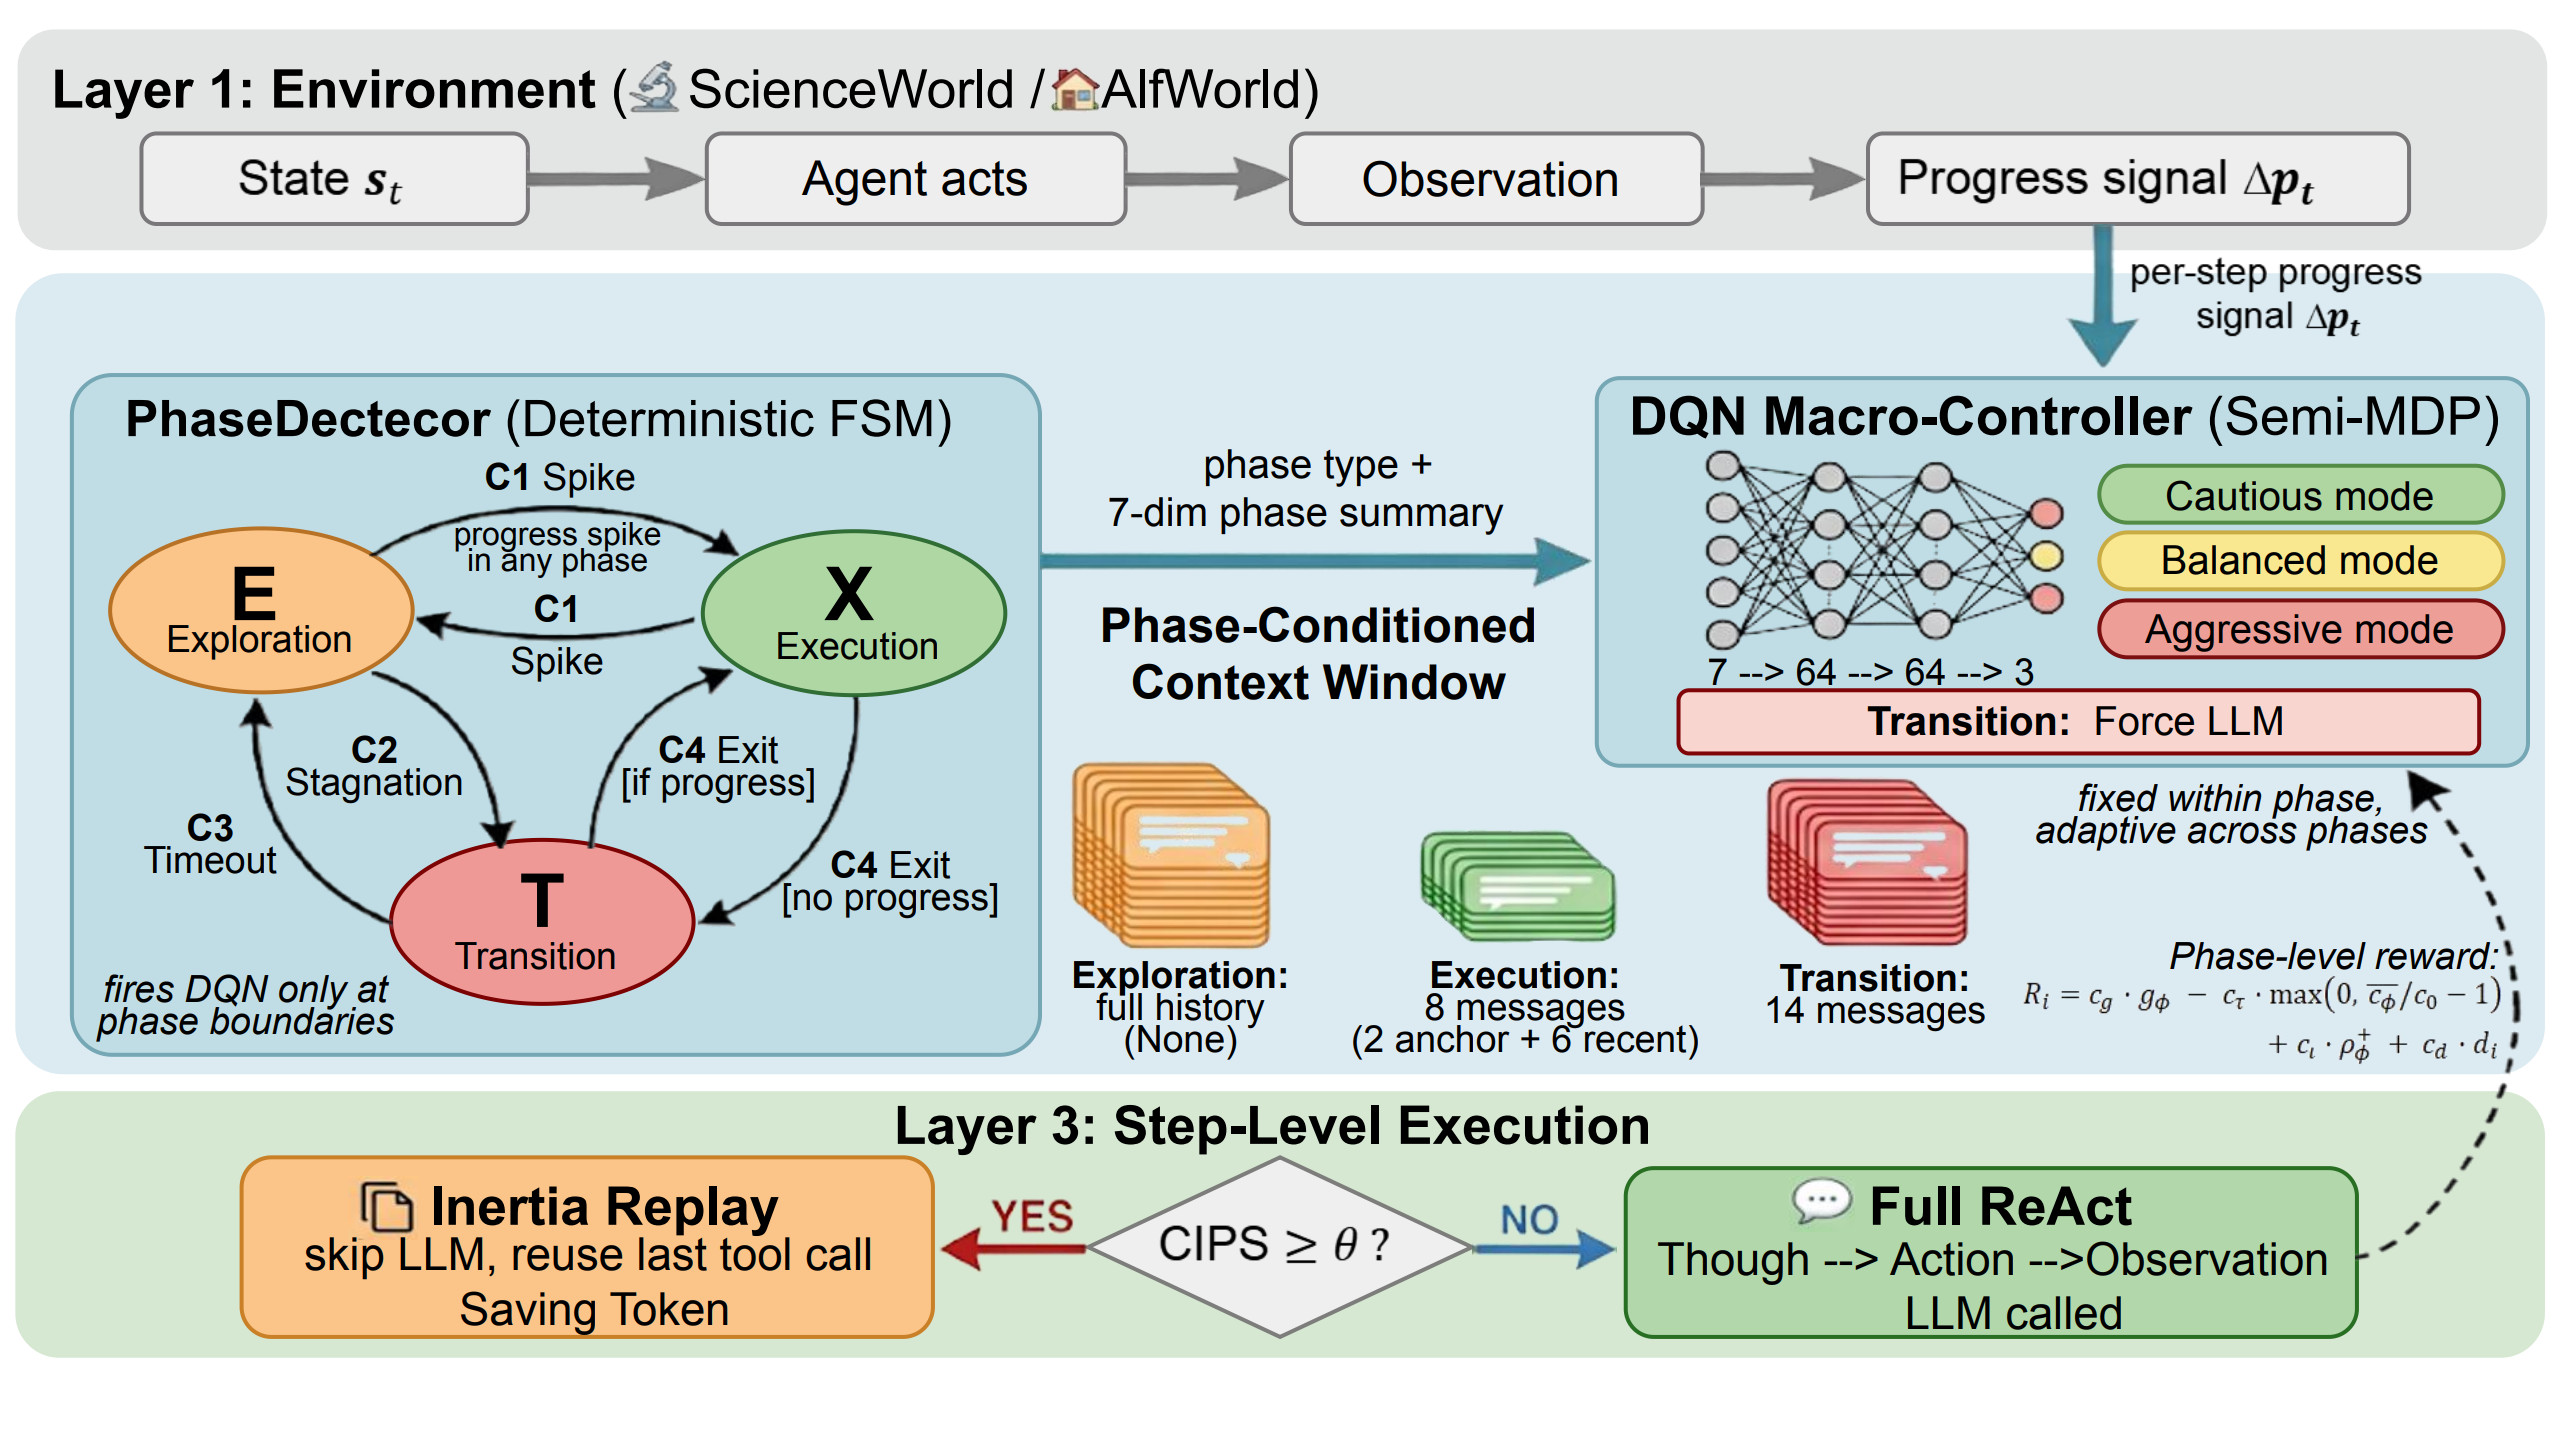
\includegraphics[width=\linewidth]{images/method.pdf}
    \caption{TEMPO: a deterministic PhaseDetector FSM identifies semantic phase boundaries; a Semi-MDP DQN macro-controller selects phase-level inertia thresholds at each boundary.}
    \label{fig:overview}
\end{figure}
\subsection{Preliminaries: AutoTool and Fixed-Threshold Inertia}
\label{sec:background}
\textbf{AutoTool}~\cite{autotool} models tool-usage patterns via a Tool Inertia Graph (TIG) $G=(V,E)$ and computes a Contextual Inertia Prediction Score at each step $t$:
\begin{equation}
  \mathrm{CIPS}(t) = (1-\alpha)\,S_{\mathrm{freq}}(t) + \alpha\,S_{\mathrm{ctx}}(t),
  \label{eq:cips}
\end{equation}
where $S_{\mathrm{freq}}$ captures tool-transition frequency from the TIG, $S_{\mathrm{ctx}}$ measures contextual semantic similarity, and $\alpha$ is a mixing coefficient.
When $\mathrm{CIPS}(t)\ge\theta$ (fixed threshold $\theta=0.1$), the previous tool call is replayed (\emph{inertia}), bypassing LLM inference; otherwise the agent falls back to full ReAct~\cite{react} reasoning.
AutoTool further enforces a hard 30\% inertia cap and prohibits consecutive inertia calls.

However, a single static $\theta$ cannot accommodate the qualitatively different behavioural regimes within a trajectory: during early exploration a low threshold triggers inertia before a coherent plan has formed; during confident execution the hard cap suppresses beneficial bypasses; at sub-task boundaries any inertia risks perpetuating an outdated action.
These failure modes motivate a phase-aware, adaptive scheduling policy.


\subsection{Phase Detection: Deterministic Finite-State Machine}
\label{sec:phase_detector}
We observe that agent trajectories naturally decompose into three recurring phases, each with distinct inertia requirements:

  \textbf{Exploration ($\mathcal{E}$)}: low-confidence information gathering; inertia is \emph{cautious} to avoid premature commitment.
  \textbf{Execution ($\mathcal{X}$)}: confident plan execution; inertia can be \emph{aggressive} to maximise token savings.
  \textbf{Transition ($\mathcal{T}$)}: a progress spike signals sub-task completion; the LLM is \emph{forced} to re-plan via $\theta_{\max}=1.5$ (exceeding the maximum possible CIPS, making inertia impossible).


\textbf{PhaseDetector} implements phase detection as a deterministic FSM with four transition rules evaluated in priority order:

\begin{itemize}
  \item \textbf{C1 (Progress spike).} If $\Delta p_t \ge \xi$ in \emph{any} phase, a sub-task has just completed; immediately enter $\mathcal{T}$ for a cooldown of $W_{\mathrm{trans}}$ steps.
  \item \textbf{C2 (Stagnation).} If in $\mathcal{X}$ with no progress for $W_{\mathrm{stag}}$ consecutive steps, the plan has likely failed; switch to $\mathcal{E}$.
  \item \textbf{C3 (Exploration timeout).} If in $\mathcal{E}$ for more than $W_{\mathrm{explore}}$ steps, force entry into $\mathcal{X}$ to prevent indefinite hesitation.
  \item \textbf{C4 (Transition end).} When the cooldown expires, enter $\mathcal{X}$ if the re-planning step made progress, otherwise enter $\mathcal{E}$.
\end{itemize}

Hyperparameters $(\xi, W_{\mathrm{stag}}, W_{\mathrm{trans}}, W_{\mathrm{explore}})$ are tuned per environment; values are reported in Section~\ref{sec:impl}.

% \begin{table}[h]
%   \centering
%   \caption{PhaseDetector hyperparameters. Bold values differ from the default.}
%   \label{tab:phase_params}
%   \small
%   \begin{tabular}{lccc p{4.5cm}}
%     \toprule
%     Parameter & Default & ScienceWorld & AlfWorld & Role \\
%     \midrule
%     $W_{\mathrm{stag}}$    & 5    & 4    & \textbf{8}    & Steps without progress before entering $\mathcal{E}$ \\
%     $W_{\mathrm{trans}}$   & 2    & 2    & 2             & Cooldown length in $\mathcal{T}$ \\
%     $W_{\mathrm{explore}}$ & 8    & 7    & \textbf{3}    & Max steps in $\mathcal{E}$ before forcing $\mathcal{X}$ \\
%     $\xi$                  & 0.05 & 0.05 & \textbf{0.01} & Progress spike threshold \\
%     \bottomrule
%   \end{tabular}
% \end{table}

\subsection{Semi-MDP Formulation}
\label{sec:smdp}
We model inertia threshold selection as a \textbf{Semi-Markov Decision Process} (Semi-MDP) $\mathcal{M}=(\mathcal{S},\mathcal{A},\mathcal{P},\mathcal{R},\gamma)$, where decisions are made only at \emph{phase boundaries} rather than at every step.
This is the key distinction from flat MDP approaches: each decision persists for an entire phase (5--8 steps), and the holding time $\tau_\phi$ is determined by environment dynamics rather than fixed in advance.
The number of macro-decisions per episode is approximately $1/6$ of the total step count, substantially reducing the RL sample burden.

\textbf{State.} At each phase boundary the controller receives a 7-dimensional summary of the just-completed phase:
$$\mathbf{s} = \left[\tfrac{\phi}{2},\; g_\phi,\; \rho_\phi,\; \tfrac{\ell_\phi}{T},\; \eta_\phi,\; \tfrac{T-t}{T},\; p_t\right]^\top \in [0,1]^7,$$
encoding phase type, progress gain $g_\phi$, inertia ratio $\rho_\phi$, relative phase length, per-step efficiency $\eta_\phi$, remaining budget, and cumulative progress—enabling credit assignment over the full phase rather than a single step.

\textbf{Actions.} The macro-controller selects from three phase-level policies: \textsc{Cautious} ($\hat\theta=0.6$), \textsc{Balanced} ($\hat\theta=0.3$), and \textsc{Aggressive} ($\hat\theta=0.1$).
The chosen threshold remains fixed throughout the phase.
During $\mathcal{T}$, the threshold is unconditionally overridden to $\theta_{\max}=1.5$ (exceeding the maximum possible CIPS score), ensuring the LLM is always invoked for re-planning regardless of the DQN output.

\textbf{Reward.} Upon phase completion, the macro-controller receives:
\begin{equation}
  R_i = c_g\cdot g_\phi \;-\; c_\tau\cdot\max\!\bigl(0,\,\bar{c}_\phi/c_0-1\bigr) \;+\; c_\iota\cdot\rho_\phi^{+} \;+\; c_d\cdot d_i,
  \label{eq:reward}
\end{equation}
where $g_\phi\!\in\![0,1]$ is the total task-progress gain over the phase; $\bar{c}_\phi$ is the mean per-step token cost against a per-step budget $c_0$; $\rho_\phi^{+}$ is the inertia precision (fraction of inertia steps yielding non-zero progress); and $d_i\!\in\!\{0,1\}$ is the task-completion indicator ($d_i{=}1$ iff the episode terminates successfully at phase $i$), providing a terminal bonus that prevents convergence to high-progress but incomplete solutions. Coefficients and $c_0$ are given in Section~\ref{sec:impl}.

The macro-controller optimises the expected discounted return over phases:
\begin{equation}
  \max_\pi\;\mathbb{E}\!\left[\sum_{i=0}^{N_\phi}\gamma^i R_i\right],
  \label{eq:objective}
\end{equation}
where $N_\phi$ is the number of phase boundaries per episode and $\gamma=0.9$.

\subsection{Macro-Controller: Semi-MDP DQN}
\label{sec:macro}
The macro-controller is a DQN trained \emph{online} during evaluation, minimising the temporal-difference loss at each phase boundary:
$$\mathcal{L} = \mathbb{E}\!\left[\!\left(R_i + \gamma(1-d_i)\max_{a'}Q(\mathbf{s}_{i+1},a') - Q(\mathbf{s}_i,a_i)\right)^{\!2}\right].$$
Starting from zero weights, the policy learns the phase-to-policy mapping across episodes without pre-training, simulating a realistic deployment scenario where the task distribution is unknown in advance. Architecture and training hyperparameters are given in Section~\ref{sec:impl}.

%% ============================================================
\subsection{Phase-Conditioned Context Management}
\label{sec:context}
%% ============================================================

Beyond threshold scheduling, TEMPO reduces token cost by trimming the LLM's conversation history per phase: a short window in $\mathcal{X}$ (plan established; recent context suffices), a medium window in $\mathcal{T}$ (sub-task context needed for re-planning), and full history in $\mathcal{E}$ (enabling reasoning over past attempts).
We additionally introduce a phase-conditioned consecutive inertia cap: more consecutive inertia calls are permitted in $\mathcal{X}$ to accommodate repetitive action chains (e.g.\ \texttt{pick\_up}$\to$\texttt{go\_to}$\to$\texttt{put\_down}), while stricter limits apply in $\mathcal{E}$ and $\mathcal{T}$ to keep the LLM involved during uncertain phases. Concrete window sizes and caps are given in Section~\ref{sec:impl}.

\subsection{Positioning}
\label{sec:comparison}
Compared with AutoTool (fixed $\theta=0.1$, hard 30\% cap, no learning) and flat-MDP approaches (dynamic $\theta_t$ at every step), TEMPO makes decisions only at phase boundaries—approximately $T/\bar{\tau}\approx T/6$ times per episode—reducing RL decision frequency by $5\text{-}8\times$. Each decision is conditioned on a 7-dimensional phase-level summary rather than instantaneous step features, replacing AutoTool's hard constraint with a phase-aware soft cap learned from experience.



\section{Experiment}
\label{sec:exp}

\subsection{Experimental Setup}
We evaluate TEMPO on two standard benchmarks for LLM agents. \textbf{ScienceWorld}~\cite{scienceworld} represents a complex scientific reasoning environment featuring non-linear state transitions and dense sub-goal progress rewards; its continuous progress signal makes it our primary platform for evaluating the Semi-MDP macro-controller's planning efficiency. \textbf{AlfWorld}~\cite{alfworld} is a text-based household manipulation benchmark whose binary terminal rewards (0 until task completion, then 1) and repetitive action chains make it a challenging testbed for inertia control: the absence of intermediate progress signals means sub-goal boundaries cannot be detected from reward alone, stressing the robustness of the PhaseDetector.

Our implementation compares TEMPO against the standard \textbf{ReAct}~\cite{react} baseline and the static \textbf{AutoTool}~\cite{autotool} framework. We utilize three frontier LLMs: \textbf{Qwen2.5-72B-Instruct}, \textbf{GPT-4o-mini}, and \textbf{GPT-3.5-Turbo}. Performance is measured through \textbf{SR} (Success Rate), \textbf{PR} (Progress Rate), and \textbf{Tokens} (total input and output consumption). All experiments are conducted with a 30-step limit and a temperature of 0 to ensure consistency.

\subsection{Implementation Details}
\label{sec:impl}

\textbf{PhaseDetector.}
ScienceWorld: $\xi{=}0.05$, $W_{\mathrm{stag}}{=}4$, $W_{\mathrm{trans}}{=}2$, $W_{\mathrm{explore}}{=}7$.
AlfWorld (binary rewards): $\xi{=}0.01$, $W_{\mathrm{stag}}{=}8$, $W_{\mathrm{trans}}{=}2$, $W_{\mathrm{explore}}{=}3$; the lower spike threshold and wider stagnation window prevent premature phase switches under reward sparsity.

\textbf{Macro-controller.}
Two-layer MLP DQN ($7{\to}64{\to}64{\to}3$); replay buffer 5000, mini-batch 64, discount $\gamma{=}0.9$. $\varepsilon$-greedy: $\varepsilon_0{=}0.3\!\to\!\varepsilon_{\min}{=}0.05$, decay 0.999 per phase boundary; Q-values stabilise after ${\approx}200$ phase boundaries (${\approx}40$ ScienceWorld episodes). Reward weights $(c_g,c_\tau,c_\iota,c_d){=}(10,2,1.5,10)$, per-step token budget $c_0{=}2000$.

\textbf{Context management.}
Window sizes: $\mathcal{X}$: 8 messages (2 context-anchoring + 6 recent); $\mathcal{T}$: 14; $\mathcal{E}$: full history. Consecutive inertia caps: $\mathcal{X}$: 4; $\mathcal{E}$ and $\mathcal{T}$: 1.

\textbf{Ablated components (Table~\ref{tab:ablation_step}).}
Three components are added incrementally: (i)~\emph{Phase Hierarchy} — FSM with static thresholds ($\hat\theta{=}0.6$ in $\mathcal{E}$, $0.3$ in $\mathcal{T}$, $0.1$ in $\mathcal{X}$); (ii)~\emph{Dynamic Intensity Switching} — static thresholds replaced by the DQN; (iii)~\emph{Phase Memory Trimming} — phase-conditioned context windows and inertia caps enabled. GPT-3.5-Turbo ($n{=}90$, ScienceWorld) is chosen as the backbone because its limited instruction-following capacity maximises the discriminable marginal contribution of each component.

\subsection{Main Results}

We primarily select \textbf{ScienceWorld} as our main evaluation testbed due to its granular feedback mechanism. To ensure statistical reliability, all reported metrics are the \textbf{average of three independent runs}. Table~\ref{tab:main} summarizes the comparative results between TEMPO and the baselines.

\begin{table}[htb]
\centering
\small
\caption{Comprehensive comparison of task performance and cost on \textbf{ScienceWorld} between TEMPO and baselines (average of three independent runs). The \textbf{Savings} column represents the token reduction of \textbf{TEMPO} relative to the \textbf{ReAct} baseline.}
\vspace{2mm}
\begin{tabular}{lccccl}
\toprule
\textbf{Base LLM} & \textbf{Method} & \textbf{SR} & \textbf{PR} & \textbf{Tokens} & \textbf{Savings}\\
\midrule
\multirow{3}{*}{Qwen2.5-72B-Instruct} & ReAct & 79.6\% & 85.0\% & 5.66M & \multirow{3}{*}{\textsl{\textbf{25.4\%}}} \\
& AutoTool & 51.8\% & 61.4\% & 3.42M & \\
& \textbf{TEMPO} & \textsl{\textbf{65.6\%}} & \textsl{\textbf{72.2\%}} & \textsl{\textbf{4.22M}} & \\
\midrule
\multirow{3}{*}{GPT-4o-mini} & ReAct & 64.4\% & 75.0\% & 7.73M & \multirow{3}{*}{\textsl{\textbf{42.9\%}}}\\
& AutoTool & 58.9\% & 73.8\% & 5.66M & \\
& \textbf{TEMPO} & \textsl{\textbf{66.7\%}} & \textsl{\textbf{75.5\%}} & \textsl{\textbf{4.41M}} & \\
\midrule
\multirow{3}{*}{GPT-3.5-Turbo} & ReAct & 64.4\% & 72.7\% & 7.36M & \multirow{3}{*}{\textsl{\textbf{42.7\%}}}\\
& AutoTool & 51.1\% & 59.4\% & 4.78M & \\
& \textbf{TEMPO} & \textsl{\textbf{66.7\%}} & \textsl{\textbf{75.9\%}} & \textsl{\textbf{4.22M}} & \\
\bottomrule
\end{tabular}
\label{tab:main}
\end{table}

On ScienceWorld, TEMPO consistently outperforms AutoTool while improving token efficiency. For Qwen2.5-72B, the FSM-based phase detection eliminates "phase-blind" re-planning failures at sub-goal boundaries, recovering SR from 51.8\% to 65.6\%. For GPT-4o-mini and GPT-3.5-Turbo, TEMPO achieves true Pareto improvements, surpassing the ReAct baseline in SR while saving up to 42.9\% in tokens—confirming that externalising inertia control to a deterministic phase hierarchy acts as a reasoning regulariser, preventing LLM over-thinking during routine execution steps.

Notably, TEMPO's hierarchical design drastically reduces the macro-controller's decision frequency. While a flat MDP would require 30 decisions per episode, TEMPO only triggers the DQN at phase boundaries, resulting in an average of only 4.8 macro-decisions per task (a 6.25$\times$ reduction). This temporal abstraction not only stabilizes the learning process but also ensures strategy consistency during extended sequences. 

Furthermore, TEMPO demonstrates strong cross-dataset generalizability across AlfWorld and PDDL (refer to Appendix~\ref{appendix:details}). We also provide a head-to-head comparison with the dual-system agent SwiftSage \cite{swiftsage} in the Appendix, which further highlights TEMPO's efficiency in balancing performance with computational overhead compared to traditional model-switching architectures. The one observed limitation occurs with GPT-3.5-Turbo on AlfWorld, where sparse terminal rewards hinder progress-spike detection, a phenomenon analyzed in our Appendix.



\subsection{Ablation Study}

We evaluate the contribution of each component within \textbf{TEMPO} on ScienceWorld using GPT-3.5-Turbo ($n=90$). The results, summarized in Table \ref{tab:ablation_step}, reflect the incremental performance gains as the framework is constructed.

\begin{table}[htb]
\centering
\small
\caption{Step-by-step ablation study on ScienceWorld (GPT-3.5-Turbo, $n=90$).}
\label{tab:ablation_step}
\begin{tabular}{lcccc}
\toprule
\textbf{Variant} & \textbf{SR} & \textbf{PR} & \textbf{Avg. Tokens} & \textbf{LLM Calls} \\
\midrule
ReAct & 64.4\% & 72.7\% & 82,494 & 17.9 \\
AutoTool & 51.1\% & 59.4\% & 54,048 & 12.4 \\
\midrule
+ Phase Hierarchy (Static Inertia) & 63.3\% & 74.9\% & 53,015 & 13.9 \\
+ Dynamic Intensity Switching & \textbf{70.0\%} & \textbf{77.5\%} & 55,167 & 14.6 \\
+ Phase Memory Trimming (Full Model) & 66.7\% & 75.9\% & \textbf{48,047} & \textbf{13.4} \\
\bottomrule
\end{tabular}
\end{table}

Flat inertia (AutoTool) collapses SR to 51.1\% on GPT-3.5-Turbo—below the no-inertia ReAct baseline of 64.4\%—because a model with limited instruction-following capacity cannot self-determine when to exit the inertia chain. Adding the Phase Hierarchy (FSM) recovers SR to 63.3\% by making this decision deterministically, and the learned DQN pushes it further to 70.0\%. Phase Memory Trimming then trades a small SR decrease (70.0\%$\to$66.7\%) for a 12.9\% token reduction, as aggressive $\mathcal{X}$-phase truncation discards some task-critical history for a model with weak in-context recall. For stronger models (GPT-4o-mini), the full TEMPO pipeline surpasses the ReAct baseline in SR (66.7\% vs.\ 64.4\% on ScienceWorld), suggesting trimming is less harmful when the model has higher in-context recall capacity; this component should therefore be selectively enabled based on model capability.

\subsubsection{Macro-Controller Efficiency: DQN vs. Rule-based}

To verify the necessity of the learned Macro-Controller, we compare our DQN-based approach against a rule-based baseline in Table \ref{tab:rule_vs_dqn}.

\begin{table}[htb]
\centering
\small
\caption{Comparison of Macro-Controller Policy: DQN vs.\ rule-based threshold selection (ScienceWorld, GPT-3.5-Turbo). Both variants use the same PhaseDetector FSM.}
\label{tab:rule_vs_dqn}
\begin{tabular}{lcccc}
\toprule
\textbf{Macro-Controller} & \textbf{SR} & \textbf{PR} & \textbf{Avg. Tokens} & \textbf{LLM Calls} \\
\midrule
Rule-based Baseline & 66.7\% & 75.1\% & 60,750 & 16.8 \\
DQN (Full Model) & 66.7\% & \textbf{75.9\%} & \textbf{48,047} & \textbf{13.4} \\
\bottomrule
\end{tabular}
\end{table}

Both methods share the same FSM and achieve equal SR, confirming that phase detection alone captures the key structural signal. The DQN's advantage lies in \emph{which} threshold it selects: where the rule-based baseline statically maps Exploration$\to\theta{=}0.6$ and Execution$\to\theta{=}0.1$, the DQN adapts based on the 7-dimensional phase summary—choosing more aggressive strategies when prior-phase efficiency is high—thereby cutting token consumption by 20.9\% and LLM calls by 3.4 per episode.

\subsection{Long-Horizon Performance Analysis}

Figure~\ref{fig:pr_n_curves} illustrates the average progress rate at different step budgets ($PR@N$) for the three methods. $PR@N$ is defined as the average progress rate achievable when the agent's maximum steps are limited to $N$, measuring the task completion efficiency under a limited interaction budget.

Three stages are visible. \textbf{Stage 1} ($N<20$): ReAct leads TEMPO by ${\approx}6.2$ pp at $N=15$, as the agent intentionally maintains low inertia during Exploration. \textbf{Stage 2} ($20\le N<25$): TEMPO closes the gap upon entering the Execution phase, accelerating through predictable tool sequences. \textbf{Stage 3} ($N\ge 25$): TEMPO significantly outperforms both baselines as the DQN has accumulated sufficient experience to select aggressive strategies reliably—demonstrating TEMPO's compounding advantage in long-horizon tasks.


\begin{figure}[htb]
	\centering
	\includegraphics[width=0.8\linewidth]{images/Long-Horizon-Performance-Analysis.pdf}
    \caption{Long-horizon performance efficiency analysis on ScienceWorld.}
    \label{fig:pr_n_curves}
\end{figure}
\subsection{Phase Behavior Visualization}

We visualize the phase transition behavior of TEMPO in a representative AlfWorld task ("pick and place") to qualitatively assess the FSM logic. As shown in Figure~\ref{fig:vis}, the agent correctly transitions from \textit{Exploration} to \textit{Execution} once the target object's location is identified. 

Crucially, the \textit{Transition} phase is triggered immediately upon the first successful "pick" action (a progress spike). This forces the LLM to consolidate the current plan and generate a new high-level instruction for the "place" sub-goal. Unlike AutoTool, which might erroneously apply inertia to the next action based on context similarity, TEMPO's FSM ensures that critical sub-goal boundaries are always handled by a fresh LLM call, directly contributing to the recovery of success rates in frontier models.

\begin{figure}[htb]
	\centering
	\includegraphics[width=0.8\linewidth]{images/Phase-Behavior-Visualization.pdf}
    \caption{Qualitative analysis of phase transitions and inertia triggering.}
    \label{fig:vis}
\end{figure}
\section{Conclusion}
We presented \textbf{TEMPO}, a hierarchical reinforcement learning framework that replaces AutoTool's static inertia threshold with a two-level architecture.
A deterministic three-state FSM (\textsc{PhaseDetector}) segments each trajectory into Exploration, Execution, and Transition phases by monitoring per-step progress signals.
A Semi-MDP DQN (Macro-Controller) then selects a phase-level inertia strategy at every FSM-triggered boundary, committing to it for the entire phase duration.

This design confers three concrete advantages: (1) operating at phase boundaries reduces RL decision frequency by 5--8$\times$ and provides denser credit assignment via phase-aggregated rewards, overcoming the sparse-reward bottleneck common in flat step-level approaches; (2) phase-conditioned context trimming reduces token overhead during Execution phases without degrading reasoning quality during Exploration or Transition; (3) the unconditional LLM invocation in the Transition phase prevents the performance collapse caused by AutoTool's phase-blind inertia at sub-task boundaries.

Experiments on ScienceWorld and AlfWorld across Qwen2.5-72B, GPT-4o-mini, and GPT-3.5-Turbo show that TEMPO consistently improves success rate over AutoTool on ScienceWorld while reducing token consumption by up to 42.9\%. On AlfWorld, TEMPO improves over AutoTool for stronger models where sparse-reward adaptation is sufficient, though GPT-3.5-Turbo's limited instruction-following capability means binary-reward environments remain a harder case. These results confirm that explicit phase detection combined with Semi-MDP temporal abstraction is an effective and general approach to adaptive inertia scheduling in LLM agents, with future work needed to improve robustness under sparse-reward conditions.

\begin{thebibliography}{99}

\bibitem{gpt4}
OpenAI: GPT-4 technical report. arXiv preprint \href{https://arxiv.org/abs/2303.08774}{arXiv:2303.08774} (2023)

\bibitem{llama3}
Grattafiori, A., Dubey, A., Jauhri, A., et al.: The Llama 3 herd of models. arXiv preprint \href{https://arxiv.org/abs/2407.21783}{arXiv:2407.21783} (2024)

% \bibitem{llama2}
% Touvron, H., Martin, L., Stone, K., et al.: Llama 2: open foundation and fine-tuned chat models. arXiv preprint \href{https://arxiv.org/abs/2307.09288}{arXiv:2307.09288} (2023)

\bibitem{react}
Yao, S., Zhao, J., Yu, D., et al.: ReAct: synergizing reasoning and acting in language models. In: ICLR (2023)

\bibitem{agentboard}
Ma, C., Zhang, J., Zhu, Z., et al.: AgentBoard: an analytical evaluation board of multi-turn LLM agents. In: NeurIPS (Datasets and Benchmarks Track). (2024)

\bibitem{deepseekr1}
DeepSeek-AI: DeepSeek-R1: incentivizing reasoning capability in LLMs via reinforcement learning. arXiv preprint \href{https://arxiv.org/abs/2501.12948}{arXiv:2501.12948} (2025)

\bibitem{bot}
Ding, Z., et al.: Buffer of Thoughts: thought-augmented reasoning with a meta-buffer. In: NeurIPS (2024)

\bibitem{agentflan}
Chen, Z., Liu, K., Wang, Q., et al.: Agent-FLAN: designing data and methods of effective agent tuning for large language models. In: Findings of the ACL: ACL 2024. pp. 9354--9366. ACL (2024)

\bibitem{swiftsage}
Lin, B.Y., Fu, Y., Yang, K., et al.: SwiftSage: a generative agent with fast and slow thinking for complex interactive tasks. In: NeurIPS (2023)

\bibitem{autotool}
Jia, J., Li, Q.: AutoTool: efficient tool selection for large language model agents. In: AAAI (2026)

\bibitem{agentlite}
Liu, Z., Yao, W., Zhang, J., et al.: Agent-lite: a lightweight library for building and accelerating multi-agent systems. arXiv preprint \href{https://arxiv.org/abs/2402.15538}{arXiv:2402.15538} (2023)

\bibitem{sutton1999between}
Sutton, R.S., Precup, D., Singh, S.: Between MDPs and semi-MDPs: a framework for temporal abstraction in reinforcement learning. Artif. Intell. \textbf{112}(1--2), 181--211 (1999)

\bibitem{toolllm}
Qin, Y., Liang, S., Ye, Y., et al.: ToolLLM: facilitating large language models to master 16000+ real-world APIs. In: ICLR (2024)

\bibitem{toolformer}
Schick, T., Dwivedi-Yu, J., Dessì, R., et al.: Toolformer: language models can teach themselves to use tools. In: NeurIPS (2023)

\bibitem{coa}
Gao, S., Dwivedi-Yu, J., Yu, P., et al.: Efficient Tool Use with Chain-of-Abstraction Reasoning. In: EMNLP (2024)

\bibitem{routellm}
Ong, I., Almahairi, A., Wu, V., et al.: RouteLLM: learning to route LLMs with RL. In: ICLR (2025)

\bibitem{dots}
Yue, M., Yao, W., Mi, H., Yu, D., Yao, Z., Yu, D.: DOTS: learning to reason dynamically in LLMs via optimal reasoning trajectories search. In: ICLR (2025)

\bibitem{alfworld}
Shridhar, M., Yuan, X., Côté, M.A., et al.: ALFWorld: aligning text and embodied environments for interactive learning. In: ICLR (2021)

\bibitem{scienceworld}
Wang, R., Jansen, P., Côté, M.A., et al.: ScienceWorld: is your agent smarter than a 5th grader? In: EMNLP. pp. 11279--11298. ACL (2022)

\end{thebibliography}    

\clearpage
\appendix
\section{Detailed Results on AlfWorld and PDDL}
\label{appendix:details}

To further validate the generalizability of TEMPO, we present detailed performance comparisons on two additional benchmarks: \textbf{AlfWorld} (134 examples) and \textbf{PDDL} (60 examples). These environments represent distinct task dynamics—text-based household manipulation with binary rewards versus formal logical planning with constraint satisfaction—and together they stress-test the PhaseDetector and macro-controller under conditions that differ substantially from ScienceWorld's dense sub-goal rewards.

\subsection{AlfWorld Results}
Table~\ref{tab:alfworld_detailed} presents the comprehensive evaluation on AlfWorld. Unlike ScienceWorld, AlfWorld provides only binary terminal rewards (0 until the task is fully completed, then 1). This poses a fundamental challenge for the PhaseDetector: the progress-spike trigger (condition C1) cannot rely on dense reward increments, so phase boundaries must be inferred solely from stagnation and timeout signals (C2--C4). Despite this limitation, TEMPO delivers meaningful improvements for frontier models.

For \textbf{Qwen2.5-72B}, AutoTool's static threshold causes a catastrophic SR drop (86.9\%$\to$65.7\%), because its phase-blind inertia replays outdated actions at sub-task boundaries (e.g.\ continuing \texttt{go\_to} after a successful \texttt{pick\_up}). TEMPO partially recovers SR to 73.9\% while still saving 18.7\% in tokens, demonstrating that deterministic phase detection alone can prevent the worst failure modes even under reward sparsity. For \textbf{GPT-4o-mini}, a similar pattern holds: TEMPO recovers SR from 49.6\% (AutoTool) to 52.2\% with a substantial 41.1\% token reduction.

For \textbf{GPT-3.5-Turbo}, which starts from a high ReAct baseline (SR 92.5\%), TEMPO achieves the greatest token savings (53.5\%) but incurs an SR reduction below AutoTool (57.3\% vs.\ 61.9\%). Two factors explain this: (i)~AlfWorld's binary rewards prevent reliable progress-spike detection, causing the FSM to occasionally misclassify phase boundaries; (ii)~GPT-3.5-Turbo's limited in-context recall makes it more sensitive to the aggressive $\mathcal{X}$-phase context trimming that discards task-critical history. This finding is consistent with the ScienceWorld ablation (Table~\ref{tab:ablation_step}), where Phase Memory Trimming also caused a small SR drop for GPT-3.5-Turbo. In practice, the context trimming component should be selectively disabled for weaker models in sparse-reward environments.

\begin{table}[htb]
\centering
\small
\caption{Detailed performance comparison on the AlfWorld benchmark (134 examples).}
\label{tab:alfworld_detailed}
\vspace{2mm}
\begin{tabular}{lccccc}
\toprule
\textbf{Base LLM} & \textbf{Method} & \textbf{SR} & \textbf{PR} & \textbf{Tokens} & \textbf{Savings}\\
\midrule
\multirow{3}{*}{Qwen2.5-72B-Instruct} & ReAct & 86.9\% & 86.9\% & 6.25M & \multirow{3}{*}{\textsl{\textbf{18.7\%}}} \\
& AutoTool & 65.7\% & 65.6\% & 4.10M & \\
& \textbf{TEMPO} & \textsl{\textbf{73.9\%}} & \textsl{\textbf{73.9\%}} & \textsl{\textbf{5.08M}} & \\
\midrule
\multirow{3}{*}{GPT-4o-mini} & ReAct & 59.7\% & 60.0\% & 17.00M & \multirow{3}{*}{\textsl{\textbf{41.1\%}}}\\
& AutoTool & 49.6\% & 50.5\% & 12.85M & \\
& \textbf{TEMPO} & \textsl{\textbf{52.2\%}} & \textsl{\textbf{52.7\%}} & \textsl{\textbf{10.02M}} & \\
\midrule
\multirow{3}{*}{GPT-3.5-Turbo} & ReAct & 92.5\% & 92.6\% & 14.43M & \multirow{3}{*}{\textsl{\textbf{53.5\%}}}\\
& AutoTool & 61.9\% & 62.2\% & 7.69M & \\
& \textbf{TEMPO} & \textsl{\textbf{57.3\%}} & \textsl{\textbf{57.5\%}} & \textsl{\textbf{6.71M}} & \\
\bottomrule
\end{tabular}
\end{table}

\subsection{PDDL Results}
Table~\ref{tab:pddl_detailed} summarizes the results on formal planning tasks. PDDL environments require strict logical consistency at every step: each action must satisfy preconditions and advance toward a goal state without violating any constraint. This makes them highly sensitive to incorrect action reuse—a single erroneous inertia replay can produce an invalid state from which recovery is impossible.

TEMPO demonstrates clear planning superiority: Qwen2.5-72B SR improves from 25.0\% (ReAct) to 40.0\% (+15.0 percentage points), and GPT-4o-mini improves from 25.0\% to 30.0\% (+5.0 pp). Notably, AutoTool provides no SR benefit on PDDL (25.0\% for both models), confirming that static inertia is entirely unsuitable for constraint-satisfaction tasks where action sequences are rarely repetitive. TEMPO's FSM-triggered Transition phase forces the LLM to re-evaluate the plan at sub-goal boundaries, which is precisely what these tasks require.

GPT-3.5-Turbo is excluded from the PDDL evaluation because its limited logical-consistency capacity produced near-zero SR across all methods (ReAct, AutoTool, and TEMPO alike), making the comparison uninformative.

\textbf{Token cost trade-off.} Unlike ScienceWorld, TEMPO incurs \emph{higher} token costs on PDDL ($-20.6\%$ and $-48.8\%$ ``savings''). Two factors explain this: (i)~PDDL tasks involve extensive constraint-satisfaction reasoning at each step, leaving few opportunities for inertia bypasses—most steps genuinely require LLM deliberation; (ii)~the forced LLM invocations at every Transition boundary add overhead that does not exist in the baselines. This overhead pays off handsomely in SR but not in token efficiency—an expected and acceptable trade-off for environments where logical correctness dominates over execution speed. The result also highlights an important design insight: TEMPO's value proposition varies by environment type; in reasoning-heavy domains, the primary benefit is improved SR rather than token savings.

\begin{table}[htb]
\centering
\small
\caption{Performance results on formal planning tasks (PDDL, 60 examples).}
\label{tab:pddl_detailed}
\vspace{2mm}
\begin{tabular}{lccccc}
\toprule
\textbf{Base LLM} & \textbf{Method} & \textbf{SR} & \textbf{PR} & \textbf{Tokens} & \textbf{Savings}\\
\midrule
\multirow{3}{*}{Qwen2.5-72B-Instruct} & ReAct & 25.0\% & 46.7\% & 2.72M & \multirow{3}{*}{\textsl{\textbf{-20.6\%}}} \\
& AutoTool & 25.0\% & 43.7\% & 2.70M & \\
& \textbf{TEMPO} & \textsl{\textbf{40.0\%}} & \textsl{\textbf{56.6\%}} & \textsl{\textbf{3.28M}} & \\
\midrule
\multirow{3}{*}{GPT-4o-mini} & ReAct & 25.0\% & 43.6\% & 2.42M & \multirow{3}{*}{\textsl{\textbf{-48.8\%}}}\\
& AutoTool & 25.0\% & 45.0\% & 2.39M & \\
& \textbf{TEMPO} & \textsl{\textbf{30.0\%}} & \textsl{\textbf{49.3\%}} & \textsl{\textbf{3.60M}} & \\
\bottomrule
\end{tabular}
\end{table}

\subsection{Comparison with Dual-System Agents: SwiftSage}
We compare TEMPO with SwiftSage \cite{swiftsage}, a state-of-the-art dual-system agent inspired by dual-process theory (Kahneman's System 1/System 2). SwiftSage routes each decision between a small ``Swift'' model (System 1, for intuitive actions) and a large ``Sage'' LLM (System 2, for complex planning), switching dynamically based on action confidence. Table~\ref{tab:swige} presents the results on ScienceWorld using GPT-4o-mini as the backbone for both SwiftSage's System 2 and TEMPO.

\begin{table}[H]
\centering
\small
\caption{Comparison with SwiftSage on ScienceWorld (GPT-4o-mini).}
\label{tab:swige}
\vspace{2mm}
\begin{tabular}{lccc}
\toprule
\textbf{Method} & \textbf{SR} & \textbf{PR} & \textbf{Tokens} \\
\midrule
SwiftSage \cite{swiftsage} & 65.6\% & \textbf{78.8\%} & 12.05M\\
\textbf{TEMPO (Ours)} & \textbf{66.7\%} & 75.5\% & \textbf{4.41M} \\
\bottomrule
\end{tabular}
\end{table}

As shown in Table~\ref{tab:swige}, while SwiftSage achieves a higher Progress Rate (PR: 78.8\% vs.\ 75.5\%) owing to its frequent System 2 deliberations, it incurs a massive token cost (12.05M). In contrast, TEMPO achieves a higher Success Rate (SR: 66.7\% vs.\ 65.6\%) while consuming over 63\% fewer tokens (4.41M vs.\ 12.05M).

The comparison reveals a fundamental architectural distinction. SwiftSage's dual-model design requires maintaining and routing between two separate models, incurring overhead from both the routing mechanism and the larger System 2 model's frequent invocations. TEMPO, by contrast, operates with a single LLM backbone and achieves cost savings through \emph{temporal} rather than \emph{model-level} abstraction: instead of switching between models, it decides \emph{when} to invoke the model at all. This makes TEMPO both simpler to deploy (no auxiliary model needed) and more token-efficient, demonstrating that phase-aware inertia control provides a more cost-effective alternative to traditional dual-system model switching.

\end{document}